\Chapter{A dokumentum strukturális elemzése}

Elkészítettem egy olyan programot, amely beolvassa a megadott PDF dokumentumot, majd az oldalait PNG kiterjesztésű képpé konvertálja és lementi a megadott mappába.
Ez a programban a következőképpen hajtható végre.

\begin{python}
images = convert_from_path('pdf_files/testpdf.pdf')
numberOfPages = len(images)
for i in range(numberOfPages):
    images[i].save('images/test' + format(i) + '.png', 'PNG')
\end{python}

Amint megvannak az oldalak, beolvassa őket, majd fekete-fehér képpé alakítja mindegyiket. Kezdeti lépésnek a margók levágását majd a paragrafusokra bontást, később pedig a sorokra, szavakra, majd betűkre bontás volt a cél. Jelenleg a paragrafusokra bontás már stabilan működik.

Ahhoz, hogy meg tudjam állapítani, hogy hol kezdődik a szöveg, és hol található összefüggő fehér rész (margó, sorköz stb.), intenzitást kellett számolnom a kép minden sorára és oszlopára (255: fehér, 0: fekete). Ehhez összeadtam a pixelek értékeit, majd elosztottam azok számával. Ezzel eredményül kaptam egy $x$ és egy $y$ tengely menti tömböt, amelyek az oszlopok és a sorok menti intenzitás átlagokat tartalmazzák.

\begin{python}
intensity_y = img_gray.sum(axis=1) / width
intensity_x = img_gray.sum(axis=0) / height
\end{python}

Ezt a két intenzitást \aref{fig:mf_2}. ábrával szemlélteti a program, amit le is ment a megadott mappába.

\begin{figure}[h]
\centering
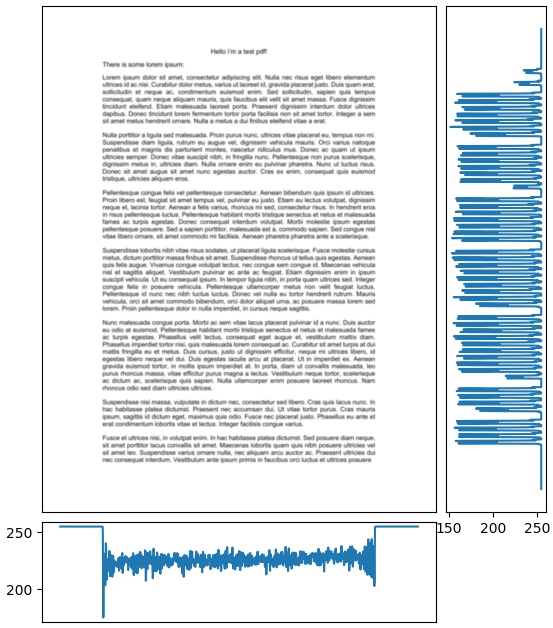
\includegraphics[scale=1]{images/mf_2.png}
\caption{A szegélyekre aggregált intenzitás értékek}
\label{fig:mf_2}
\end{figure}

Ezt a két tengely menti intenzitás tömböt felhasználva már meg lehet állapítani, melyik pixelnél ér véget a margó és hol kezdődik a szöveg. Egy egyszerű ciklussal megvizsgálom a tömb elejétől indulva hogy meddig egyenlőek az intenzitások a 255 értékkel, majd lementem azt az indexet ahol megáll a programom. Ezt megismétlem a tömbön visszafelé haladva is, így lesz meg az alsó-felső, jobb-bal margó végpontja. Ezeket felhasználva a programom eltávolítja a margókat, majd lementi a képet a megadott mappába.

\begin{python}
im1 = test.crop((left_margin,
                 height - top_margin,
                 right_margin,
                 height - bottom_margin))
im1.save('img_crop_margin/testcrop.png', 'PNG')
\end{python}

A paragrafusokra bontás is hasonlóan működik. Elindulok a tömbömön, majd egy változóban számolom hogy hány 255 értékkel egyenlő intenzitást talál egymás után a program. Ha ez több mint 10 (tapasztalati érték) akkor hozzáadja egy tömbhöz a fehér szakasz kezdőpontját (\texttt{index - 10}), majd az ehhez tartozó végpontot (amint 255 értéktől eltérő intenzitást talál, lementi az előző indexet). Így lesz egy tömböm, ami egymás után tartalmazza egy-egy bekezdésnek a kezdő majd végpontját ($y$ tengely mentén). Ezután egy ciklussal szépen kivágom a paragrafusokat.

A sorokat a paragrafusokhoz hasonlóan az eredeti képből vágom ki, de míg a paragrafusoknál mind a két oldali margót levágom, a soroknál a bal oldali margóval ezt nem teszem meg mivel erre szükségem lesz majd a szavakra bontásnál. Az algoritmus amit a paragrafusoknál használtam itt is tökéletesen működik annyi eltéréssel, hogy az egyenlő intenzitások száma legalább 2 kell legyen, hiszen maga a sorköz az kisebb mint a térköz.

Amennyiben a szövegen kívül más nem szerepel az adott oldalon, a sorokra bontáshoz nem szükséges hogy az adott oldalt felbontsuk paragrafusokra, az eredeti képből könnyedén megkaphatjuk a sorokat. Viszont ha nem tiszta (?) szöveggel van dolgunk, abban az esetben a sorokra bontás előtt szükséges megvizsgálni, hogy az oldal mely részei tartalmaznak szöveget és mely részei tartalmaznak egyéb objektumot (?). Ezt a problémát majd a későbbiekben taglaljuk.

A szavakra bontásnál szükségem van az eddig levágott sorokra, így egy for cikluson belül egyesével beolvasom őket, majd első lépésként kigyűjtöm a szavak koordinátáit. Itt már nem az y, hanem az x tengely menti intenzitást használom fel és az előző algoritmusokhoz hasonlóan a világos, 240 feletti intenzitást keresem, és amint találok belőle egymás mellett legalább 5 darabot, akkor mentem le a koordinátát. Mivel a világos részek érzékelésével keresem a szavakat, így a legelső szó elején is kell hogy legyen valamennyi világos terület hogy ne hagyja ki az algoritmus a vizsgálat során. Emiatt nem vágom le a soroknak a bal részéről a margót, mivel így biztosan megtalálja az összes szót. A másik megoldás az lehetne, hogy automatikusan lementem a 0 indexet mint kezdőindex, ezzel is biztosítva hogy a kezdeti szó koordinátái is meglegyenek, de úgy véltem hogy a margó elhagyása egy logikusabb lépés (?).

A szavak betűkre bontása már egy érdekesebb témakör. Ennél az algoritmusnál már nem a világos, hanem épp hogy a sötét részeket kerestem, és ha már 1 pixelnek megfelelő sötét részt is találtam már mentettem az adott indexet. Ez a legtöbb esetben szépen működött és megkaptam egyesével a betűket. Viszont a ligatúrák esetében a betűk egymásba lógnak, ezért az algoritmusom nem vágta szét őket, hanem egybe mentette le. Ilyen esetek voltak például az r és az f vagy t találkozása, vagy például a dupla t vagy f betűk.

\begin{figure}[H]
\centering
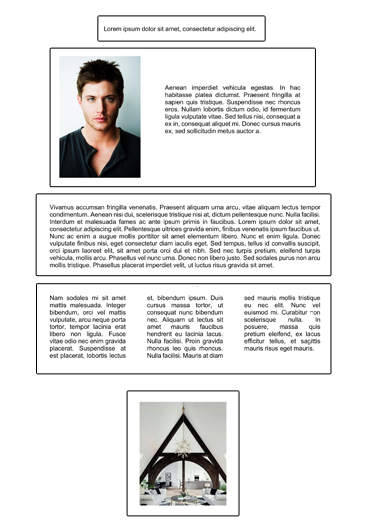
\includegraphics[scale=1]{images/page.png}
\caption{Nem csak egyszerű szöveget tartalmazó pdf}
\label{fig:page}
\end{figure}

Az eddigiekben azt feltételeztük hogy a dokumentum amelyet vizsgálunk, az szövegen kívül mást nem tartalmaz, és az adott szöveg is folytonos, egyetlen hasáb. Amennyiben egy bonyolultabb pdf dokumentumot kell feldolgoznunk (?) abban az esetben az eddigi algoritmusok a paragrafusokra bontásig működnek, ám ha a képeket (és a táblázatokat ha fogok vele foglalkozni) nem kezeljük külön, abban az esetben a sorokra bontásnál a folyamat megszakad. Annak érdekében hogy ezt elkerüljük, a paragrafusokra bontásnál egyéb vizsgálatokra van szükség.

\begin{figure}[H]
\centering
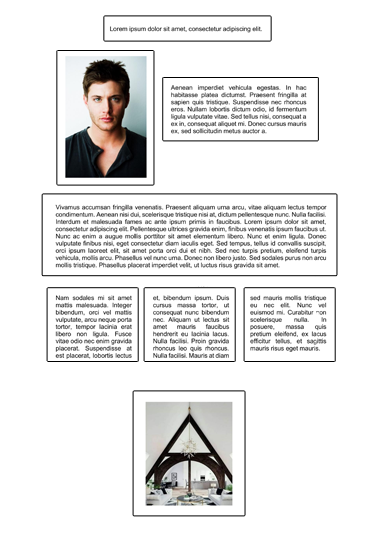
\includegraphics[scale=1]{images/page2.png}
\caption{Az egységekre bontás első szakaszának eredménye}
\label{fig:page 2}
\end{figure}

A paragrafusra bontás során a vizsgálat az y tengely mentén történik. A képek amelyeket ez úton megkapunk, vízszintesen bontják részekre a dokumentumot, tehát ha több hasábunk, vagy netalántán egy képünk van mellette valamennyi szöveggel, azok mind egy egységet alkotnak. A feladatunk hogy ezeket az egységeket szétbontsuk, és megismerjük hogy az adott részegységek szöveget tartalmaznak vagy valami mást.

A szétbontás hasonlóan működik mint az eddigi algoritmusok. Betöltjük magát a képet, végrehajtunk rajta egy intenzitás vizsgálatot méghozzá az x tengely mentén, majd ezt megvizsgálva kimentjük a fehér részek koordinátáit.

Abban az esetben, ha az algoritmus nem talál koordinátát, akkor visszatér egy hamis értékkel, és a teljes képpel dolgozik tovább.

Amennyiben talál, akkor következik a részegységekre bontás. Mivel a paragrafusoknál a bal és jobb szélső margó már nem szerepel a képen, így nincsen kezdeti fehér rész amelyből az algoritmus kiindulhatna. Ezért a koordinátákat tartalmazó lista kezdő, és végpontja a 0 és a szélesség kell legyen. Ezt a két értéket a crop (?) metódus előtt hozzáadom a listához. Amennyiben a kép vagy szöveg tartalmaz behúzást, abban az esetben az algoritmus megtalálja a jobb/bal oldali fehér részt, így a kezdeti és végpont hozzáadása már nem szükséges mivel a lista már tartalmazza azokat. Egy egyszerű if utasítással megtudom állapítani hogy szükséges-e a hozzáadás vagy sem. Ezt a megoldás a későbbiekben bevezettem a szavakra bontásnál is, hiszen így nem kell üres teürleteket kihagynom a sorokra bontás során.

\begin{figure}[H]
\centering
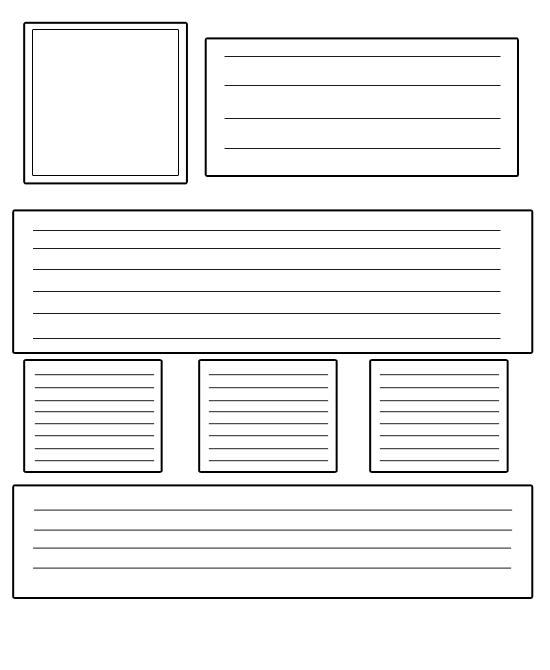
\includegraphics[scale=1]{images/page3.png}
\caption{Az egységekre bontás második szakaszának eredménye}
\label{fig:page 3}
\end{figure}

Eredményül megkaptuk a dokumentumot egységekre bontva. Ezek után már csak azt kell megvizsgálni, hogy az adott egység kép vagy szöveg, és ennek megfelelően menteni.

\begin{figure}[H]
\centering
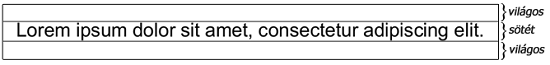
\includegraphics[scale=1]{images/line.png}
\caption{Szöveg felhasznált tulajdonsága (?)}
\label{fig:line}
\end{figure}

A vizsgálathoz azt a tényt használtam fel, hogy ha a szöveg akár csak egy sorból is áll, alatta és felette mindenképp található világos intenzitás (nem biztos hogy teljesen fehér, hiszen a szöveg vonala alá érő betűknek, mint például a p, a szára beletartozik az adott intenzitásba így az már nem tiszta fehér). Az algoritmus világos intenzitást keres elsőnek. Amint talál legalább 2 egységnyi világos területet (240 feletti intenzitás), abban az esetben az adott ponttól elindul, és megnézi hogy talál-e egybefüggő sötét területet (240 alatti intenzitás). Amennyiben igen, megvizsgálja hogy a sötét intenzitású terület után talál egy újabb fehér részt. Amennyiben erre is az a válasz hogy igen, az algoritmus arra a következtetésre jut hogy az adott egység szöveget tartalmaz, így azt a paragrafusokhoz menti, egyébként pedig a képekhez. Természetesen az algoritmus elég kezdetleges, így könnyen át lehet verni egy világos hátterű, középen sötét árnyalatú objektumot tartalmazó képpel. (lásd \ref{fig:tree}. ábra (?))

\begin{figure}[H]
\centering
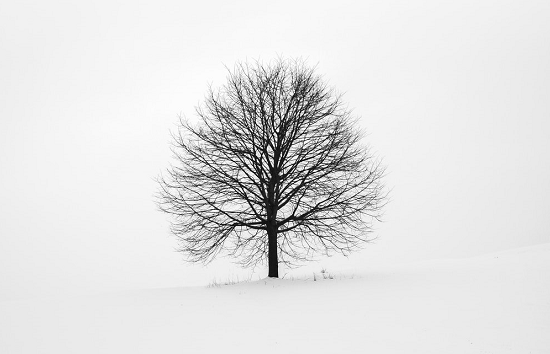
\includegraphics[scale=1]{images/tree.png}
\caption{Az algoritmus ezt a képet szövegként érzékeli}
\label{fig:tree}
\end{figure}

Az eddigi feldolgozás során a dokumentumot alulról-felfelé bontottuk részekre, viszont ahhoz, hogy végeredményként értelmes szöveget kapjunk, elengedhetetlen hogy a képek oldalhű (?) sorrendben legyenek lementve.

Mivel az intenzitás vizsgálat a lap aljáról indul, így a lista pont fordított sorrendbe tartalmazza a koordinátákat. Eddig a crop metódusban a for ciklusom a lista elejéről, most viszont a lista végéről indul el, így a lap tetején lévő paragrafus lesz lementve elsőnek, nem pedig a lap alján levő. A paragrafusokon kívül a sorok crop metódusát kellett még módosítanom, a szavakét és a karakterekét nem, mivel azokat az x tengely mentén vágom, így azok eleve megfelelő sorrenbe kerültek mentésre.

Ezzel a dokumentumom fel van bontva a legapróbb egységre (karakter) és megfelelő sorrendben követik egymást az egységek, így következhet a karakter felismerő (optical character recognition (OCR)).

A python egyik ocr eszközét (tool?) a Python-tesseract-ot hívtam segítségül (?). Első lépésben a karakter levágásnál átadtam a pytesseract \texttt{image\_to\_string} nevű metódusának a képet, majd a válaszként kapott stringet hozzá fűztem egy már meglévő stringemhez. Amint végig ért a metódus minden soron, egy külső fileba lementettem a megkapott szöveget. Sajnos azt tapasztaltam hogy az OCR egyetlen karaktert sem ismert fel.

Ebből arra következtettem hogy a felbontása az adott képnek túl alacsony lehet, így megpróbálkoztam egy nagyobb felbontású képpel, de sajnos úgy sem jártam sikerrel.

Következő lépésként egy szintet visszább léptem, és most nem a karaktereket, hanem a szavakat adtam át a metódusnak. Itt már sokkal kielégítőbb eredményt kaptam. A szavakat nagyjából 80\%-os pontossággal beazonosította, viszont itt is akadtak problémák bőven. Az egy és két betűs szavakat/kötőszavakat (pl. az, és, a, s) és a számokat nem ismerte fel a metódus (vagy csak nagyon ritkán), és üres stringeket kaptam helyettük. Ezen kívül elég sok ékezet lemaradt, és gyakran keverte a betűket, pl. I és az l esetében.

Ezen tapasztalataim után nekiláttam az ocr paramétereinek a vizsgálatához, és néhány beállítással sikerült elérnem hogy az ocr működjön karakter szinten is. Ehhez a paraméterek változtatása mellett biztosítottam, hogy az általam kivágott betűk körül mindig legyen egy fehér színű, 10 képpont méretű keret, ezzel segítve a programot a sikeresebb felismerésben. A betűtípustól függően akadnak itt is kisebb-nagyobb hibák. A word alapértelmezett Calibri betűtípusában szereplő l betű az tulajdonképpen egy vonal, így azt a program a | (AltGr + W) karakterként ismeri fel. Emellett gyakran összetéveszti a c betűt az e betűvel, a vesszőt pedig a ponttal.

Ezek természetesen az eddigi hibákhoz képest sokkal biztatóbb eredmények, és így a kapott szöveg már olvasható. 

A különböző szöveg szerkezeti egységeken való OCR használat kapcsán elvégeztem néhány tesztet. Megvizsgáltam, hogy az adott szinteken (oldal, bekezdés, sor, szó, karakter) milyen időkülönbséggel fut le a karakterfelismerő. Minden esetben a \ref{fig:mf_2}. ábra pdf dokumentumát használtam bemenetként. Ez egy egy oldalas dokumentum amely 672 szót és 4520 karaktert tartalmaz. Az eredmény a következő grafikonon látható (\ref{fig:test ocr}. ábra)

\begin{figure}[H]
\centering
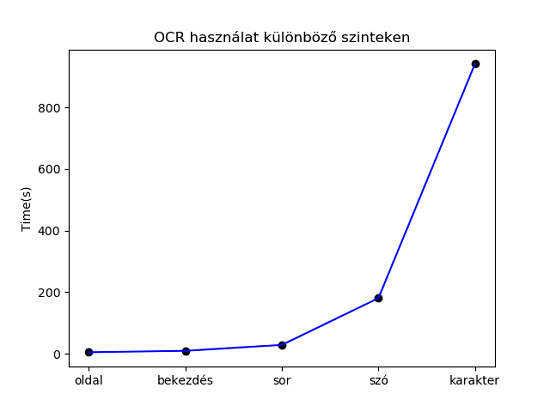
\includegraphics[scale=1]{images/test_ocr.png}
\caption{Az OCR futásának ideje másodpercben különböző szöveg szerkezeti egységeken}
\label{fig:test ocr}
\end{figure}

Amikor az ocr egy nagyobb egységet kapott feldolgozásra, akár egybe egy oldalnyi szöveget, egy bekezdést vagy csak egy sort, csekély, mindössze 5-20 másodperces különbséggel már ki is számolta(?) az eredményt. Viszont amikor már kisebb egységekkel volt dolga, sokkal több időbe telt neki mire megtalálta a legmegfelelőbb karakter. A szavaknál már olyan átlag 180 másodpercet, míg a karaktereknél ez olyan átlag 930 másodpercet vett igénybe. 

Ez a különbség főként abból adódhat, hogy bizonyos karaktereknél szüksége van az OCR-nek viszonyítási alapra, önmagában nem tudja biztosan megmondani hogy milyen karaktert kapott. Tegyük fel hogy beadunk neki egy sima 'v' betűt. Ha nincs mellette viszonyítási alap, tegyük fel egy 'a' betű, akkor a 'v' az lehet kicsi és nagy betű is. Viszont ha már egybe látja az OCR a kettő betűt, 'av' akkor már megtudja állapítani hogy a karakter az kicsi. Tapasztalatom szerint ez a szavak szintjén sem kielégítő, viszont a sorok szintjén már elég nagy pontossággal megtudja különböztetni a kis- és nagybetűket.

A tesztet elvégeztem különböző betűtípusok esetén (Calibri, Arial, Times New Roman). Arra a kérdésre kerestem a választ hogy megnehezítik-e a feldolgozást bizonyos betűtípusok vagy sem. Mint az a \ref{fig:test font}. ábrán látható, nem nagy az eltérés a különböző betűtípusok feldolgozása között. A három példa közül az Arial volt aminek a kiértékelése több időt vett igénybe minden szöveg szerkezeti egységen, de ez is nagyon csekély eltérés, így az ábrán nem is szembetűnő.

\begin{figure}[H]
\centering
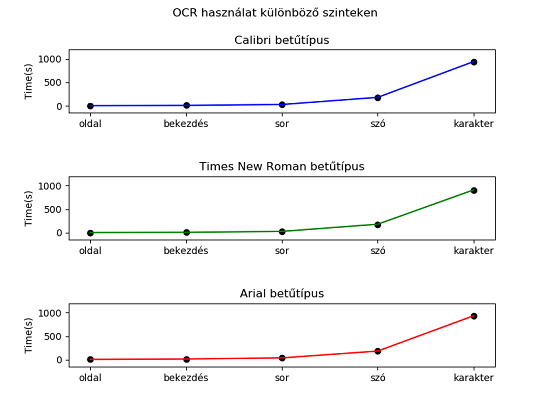
\includegraphics[scale=1]{images/test_ocr_font_types.png}
\caption{Az OCR futásának ideje betűtípusok összehasonlításával (?)}
\label{fig:test font}
\end{figure}

Azon kívül, hogy a feldolgozása a nagyobb szöveg egységeknek gyorsabb, a tesztek során az is kiderült, hogy pontosabb is. Ez első sorban a már fentebb említett karakterek egymáshoz való viszonyításának köszönhető, hiszen itt bőven akad betű amihez viszonyíthatjuk a többit. Azért a karakterek szintjén történő ocr használatát sem kell kizárni a lehetőségek közül, mivel annál is minden esetben 75\% feletti volt az eredmény pontossága. Itt a legtöbb hibát a fentebb említetten kívül az okozza, hogy különböző betűtípusokban találhatók egymásra nagyon hasonlító betűk. 